\documentclass[12pt]{article}

%\usepackage{algo}
\usepackage{tikz,fullpage,url,amssymb,amsmath,epsfig,color,xspace,alltt,mathtools}
\usetikzlibrary{shapes,chains,positioning}
\usepackage[pdftitle={CS 240 Assignment 2},%
pdfsubject={University of Waterloo, CS 240, Fall 2021},%
pdfauthor={MP}]{hyperref}
%\RequirePackage{pstricks,pst-node,pst-tree} % draw trees, requires using xetex
\newlength{\nodeLength}
\newcommand{\Node}{A}
\newcommand{\setnode}[1]{
	\settowidth{\nodeLength}{#1}
	\renewcommand{\Node}[1]{
		\Tcircle[name=#1]{\makebox[\nodeLength]{##1}}
	}
}
\setnode{99}

\newcommand{\ceil}[1]{\left\lceil #1 \right\rceil}
\newcommand{\floor}[1]{\left\lfloor #1 \right\rfloor}
\renewcommand{\thesubsection}{Problem \arabic{subsection}}

\begin{document}
	
	\begin{center}
		{\Large\bf University of Waterloo}\\
		\vspace{3mm}
		{\Large\bf CS240 Fall 2021}\\
		\vspace{2mm}
		{\Large\bf Assignment 2}\\
		\vspace{3mm}
		\textbf{Due Date: Wednesday, Oct 6 at 5:00pm}
	\end{center}
	
	\definecolor{care}{rgb}{0,0,0}
	\def\question#1{\item[\bf #1.]}
	\def\part#1{\item[\bf #1)]}
	\newcommand{\pc}[1]{\mbox{\textbf{#1}}} % pseudocode
	
	The integrity of the grade you receive in this course is very important to you and the University of Waterloo.  
	As part of every assessment in this course you must read and sign an Academic Integrity Declaration before you start working on the assessment and submit it \textbf{before the deadline of Oct 6} along with your answers to the assignment; i.e. \textbf{read, sign and submit A02-AcInDe.txt now or as soon as possible}.
	The agreement will indicate what you must do to ensure the integrity of your grade.
	If you are having difficulties with the assignment, course staff are there to help (provided it isn't last minute). \\
	~\\
	\textbf{The Academic Integrity Declaration must be signed and submitted on time or the
		assessment will not be marked.} \\
	~\\
	Please read
	\url{http://www.student.cs.uwaterloo.ca/~cs240/f21/guidelines.pdf} for guidelines on submission.  
	\textbf{Each question must be submitted individually to MarkUs as a PDF} with the corresponding file names: 
	a2q1.pdf, a2q2.pdf, ... , a2q5.pdf . 
	It is a good idea to submit questions as you go so you aren't trying to create several PDF files at the last minute. \\
	~\\
	\textbf{Late Policy:} Assignments are due at 5:00pm.
	To accommodate any small time differences with our submission server, there is a grace period of 5 minutes; i.e. we will accept assignments until 5:05pm without penalty.  Assignments submitted after 5:05pm will incur a penalty of 1 mark per minute to a maximum of 10 marks.   \\
	\textbf{Assignments submitted after 5:15pm will not be accepted}  
	but may be reviewed (by request) for feedback purposes only. \\  
	~\\
	Note: you may assume all logarithms are base 2 logarithms:  $\log = \log_2$.
	
	%%%%%%%%%%%%%%%%%%%%%%%%%%%%%%%%%%%%%%%%%%%%%%%%%%%%%%%%%%%%%
	\subsection{[4 Marks]}
	
	A \emph{stable} sorting algorithm is one in which the relative order
	of all identical elements (or keys) is the same in the output as it
	was in the input. Prove, using a well-chosen example, that heapsort is
	not a stable sorting algorithm.
	
	%%%%%%%%%%%%%%%%%%%%%%%%%%%%%%%%%%%%%%%%%%%%%%%%%%%%%%%%%%%%%
	\subsection{[3(+2)+2+4+4+6=19(+2) Marks]}
	
	A \emph{pyramid} is a data structure similar to a heap that can be used
	to implement the priority queue ADT.
	
	As with a heap, a pyramid is defined by two properties:
	\begin{itemize}
		\item \textbf{Structural property}: A pyramid $P$ consists of $\ell \geq 0$ levels. The $i$th level, for $0\leq i < \ell$, 
		contains at most $i+1$ entries, indicated as
		$P_{i,j}$ for $0\leq j\leq i$. All levels but the last are completely
		filled, and the last level is left-justified.
		
		For example, the following diagram shows the structure of a pyramid with 4 levels and 9 nodes, labelled as described above.
		
		\begin{center}
			%\usetikzlibrary{positioning}
			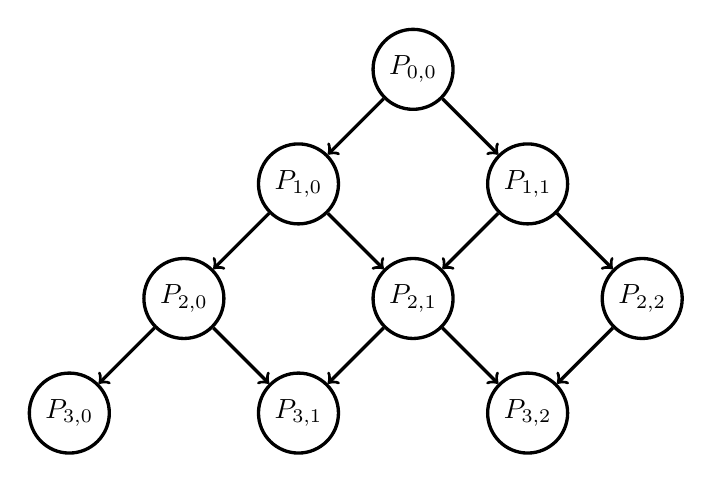
\begin{tikzpicture}[node distance=1cm,very thick]
				\node[circle,draw] (a0) {$P_{0,0}$};
				\node[circle,draw] (b0) [below left=of a0] {$P_{1,0}$};
				\node[circle,draw] (b1) [below right=of a0] {$P_{1,1}$};
				\node[circle,draw] (c0) [below left=of b0] {$P_{2,0}$};
				\node[circle,draw] (c1) [below right=of b0] {$P_{2,1}$};
				\node[circle,draw] (c2) [below right=of b1] {$P_{2,2}$};
				\node[circle,draw] (d0) [below left=of c0] {$P_{3,0}$};
				\node[circle,draw] (d1) [below right=of c0] {$P_{3,1}$};
				\node[circle,draw] (d2) [below right=of c1] {$P_{3,2}$};
				\path[->] (a0) edge (b0)
				(a0) edge (b1)
				(b0) edge (c0)
				(b0) edge (c1)
				(b1) edge (c1)
				(b1) edge (c2)
				(c0) edge (d0)
				(c0) edge (d1)
				(c1) edge (d1)
				(c1) edge (d2)
				(c2) edge (d2);
			\end{tikzpicture}
		\end{center}
		
		\item \textbf{Ordering property}: Any node $P_{i,j}$ has at most two
		\emph{children}: $P_{i+1,j}$ and $P_{i+1,j+1}$, if those nodes exist.
		The priority of a node is always greater than or equal to the priority
		of either child node.
		
		For example, the following diagram shows the ordering property for a pyramid with 4 levels and 9 nodes.  
		Priorities have been placed in the nodes and the arrows indicate ``$\geq$'' relationships.
		
		\begin{center}
			%\usetikzlibrary{positioning}
			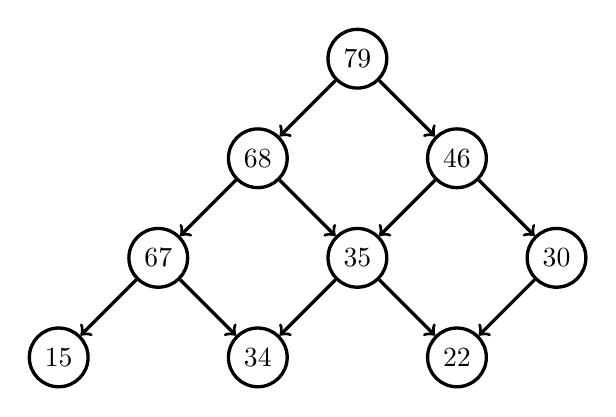
\begin{tikzpicture}[node distance=1cm,very thick]
				\node[circle,draw] (a0) {79};
				\node[circle,draw] (b0) [below left=of a0] {68};
				\node[circle,draw] (b1) [below right=of a0] {46};
				\node[circle,draw] (c0) [below left=of b0] {67};
				\node[circle,draw] (c1) [below right=of b0] {35};
				\node[circle,draw] (c2) [below right=of b1] {30};
				\node[circle,draw] (d0) [below left=of c0] {15};
				\node[circle,draw] (d1) [below right=of c0] {34};
				\node[circle,draw] (d2) [below right=of c1] {22};
				\path[->] (a0) edge (b0)
				(a0) edge (b1)
				(b0) edge (c0)
				(b0) edge (c1)
				(b1) edge (c1)
				(b1) edge (c2)
				(c0) edge (d0)
				(c0) edge (d1)
				(c1) edge (d1)
				(c1) edge (d2)
				(c2) edge (d2);
			\end{tikzpicture}
		\end{center}
	\end{itemize}
	
	\begin{itemize}
		\part{a}
		A pyramid $P$ with $n$ nodes can be stored in an array $A$ of size $n$,
		similar to an array-based heap. 
		For example, the top of the pyramid $P_{0,0}$ will be stored in $A[0]$, followed by level 1, then level 2, and so on.
		
		Give formulas for the array index that the following pyramid entries
		will have. Assume that $n$, $i$, and $j$ are such that all indicated
		pyramid nodes actually exist. You do not need to justify your answers.
		
		\begin{enumerate}
			\item $P_{i,j}$
			\item Left and right children of $P_{i,j}$
			\item Left and right parents of $P_{i,j}$
			\item (Bonus) Left and right children of the node corresponding to $A[i]$
		\end{enumerate}
		
		\part{b}
		Give upper and lower bounds for the number of nodes $n$ in a pyramid $P$
		with $\ell$ levels, where $\ell \geq 1$. For example, a pyramid with 2
		levels has at least 2 and at most 3 nodes. Your bounds should be tight.
		
		\part{c}
		Give pseudocode for the $\emph{delete-max}$ operation that takes a
		pyramid stored in an array $A$ of size $n$, removes the largest priority
		from the pyramid, and returns it.
		
		Explain why your algorithm preserves the structural and ordering properties
		of the pyramid; i.e. show that the resulting tree is a pyramid (according to
		the definition above).
		
		Show that your algorithm has time complexity $O(\sqrt{n})$.
		
		\part{d}
		Give pseudocode for the $\emph{insert}$ operation that takes a pyramid
		stored in an array $A$ of size $n$ and a priority $x$ and inserts the
		new element into the pyramid.
		
		Explain why your algorithm preserves the structural and ordering properties
		of the pyramid; i.e. show that the resulting tree is a pyramid (according to
		the definition above).
		
		Show that your algorithm has time complexity $O(\sqrt{n})$.
		
		\part{e}
		Consider the \emph{contains} problem: Given an array $A$ of size $n$
		and an number $x$, determine whether $x$ is an element of $A$.
		
		For example, if $A$ is sorted, the \emph{contains} problem can be solved in
		$O(\log n)$ time by using a binary search.
		
		Describe an efficient algorithm using pseudocode to solve the \emph{contains} problem when the input array $A$ is a pyramid as described above.  
		State and briefly describe the runtime of your algorithm.
		For full marks, your algorithm should run in $O(\sqrt{n})$.
		(Hint: A pyramid contains some sorted lists.)
		
	\end{itemize}
	
	%%%%%%%%%%%%%%%%%%%%%%%%%%%%%%%%%%%%%%%%%%%%%%%%%%%%%%%%%%%%%
	\subsection{[6 Marks]}
	
	Consider a method \emph{step-up-down} that given an array $A$ of $n$ non-repeating numbers, rearranges $A$ into blocks of varying size: the first block is size 2, the second is size 3, and so on.  Each block also orders the numbers it contains in the follow way: the first block contains numbers in decreasing order, the second block is in increasing order, the third block is in decreasing order, and so on. Adjacent blocks also have the property that the numbers in a even numbered block must all be smaller than the numbers in the immediately preceding odd numbered block.
	
	For example, given
	\begin{center}
		$A: [8,13,2,7,10,4,9,3,1]$
	\end{center}
	the output of \emph{step-up-down} could be
	\begin{center}
		$A: [13, 9, 1, 2, 3, 10, 8, 7, 4]$
	\end{center}
	Another possibly is
	\begin{center}
		$A: [13, 10, 1, 2, 3, 9, 8, 7, 4]$
	\end{center}
	
	\noindent Note: Both outputs above are valid and for a given input there may be more than one valid output. 
	Your algorithm needs to only output one valid output - any valid output is okay.
	
	\bigskip
	
	\noindent You are given two heaps (already implemented), one min-heap and one max-heap, that you may use in your implementation.
	You may use the heap methods from class without restating them here.
	The two heaps are independent (i.e. not linked) and you do not have access to their implementations.
	
	\bigskip
	
	\noindent Aside from $A$ and the two heaps, you may only use a constant amount of space.
	
	\bigskip
	
	\noindent Give pseudocode for an efficient implementation of \emph{step-up-down}.
	Also, briefly state and justify the correctness of your algorithm and its time complexity.
	
	%%%%%%%%%%%%%%%%%%%%%%%%%%%%%%%%%%%%%%%%%%%%%%%%%%%%%%%%%%%%%
	\subsection{[4+2+2+4=12 Marks]}
	
	Let $A$ be an array of $n$ distinct integers. An {\em inversion} is a pair of indices $(i, j)$ such that $i < j$ and $A[i] > A[j]$.
	\begin{enumerate}
		\part{a} Determine the maximum number and minimum number of inversions in an array of $n$ distinct integers. 
		Characterize what the arrays that attain these maxima and minima look like.
		
		\part{b} Let $A$ be an array of $n$ distinct integers chosen at random.
		Given a pair of distinct indices $i<j$, show that the probability that $(i, j)$ is an inversion is $1/2$. 
		
		\part{c} Let $A$ be an array of $n$ distinct integers chosen at random.
		Determine the expected number of inversions in an array of $n$ distinct integers. \\
		Note: You may use the result in part (b) even if you did not prove it.
		
		\part{d} Suppose a sorting algorithm is only allowed to exchange adjacent elements $(i, i + 1)$.
		Show that its worst-case and average-case complexity is $\Omega(n^2)$. \\
		Note: You may use the results from the previous parts even if you did not prove them. \\
		\textbf{Hint:} How many inversions does an exchange of adjacent elements remove?
		
	\end{enumerate}
	For parts (b-d), all permutations of the input-numbers are equally likely.
	%%%%%%%%%%%%%%%%%%%%%%%%%%%%%%%%%%%%%%%%%%%%%%%%%%%%%%%%%%%%%
	\subsection{[6 Marks]}
	
	In this question, we generalize \textit{quickSelect1} to work on two input arrays. 
	Let the resulting algorithm be called \emph{quickSelect2Arrays(A,B,k)}.
	Arrays $A$ and $B$ are of size $n$ and $m$, respectively, and $k\in \{ 0,1,...,n+m-1 \}$. 
	Algorithm \emph{quickSelect2Arrays(A,B,k)} should return the item that would be in $C[k]$ if $C$ was the array resulting from merging arrays $A$ and $B$ and $C$ was sorted in non-decreasing order. 
	
	\bigskip
	
	\noindent Your algorithm \emph{quickSelect2Arrays(A,B,k)} must be in-place, i.e. only $O(1)$ additional space is allowed.
	Briefly and informally (one or two sentences) argue that the time complexity of your algorithm is the same as of \emph{quickSelect1}, i.e. $O(v)$ in the average case where $v$ is the total number of elements in $A$ and $B$, i.e. $v=n+m$.
	
	%%%%%%%%%%%%%%%%%%%%%%%%%%%%%%%%%%%%%%%%%%%%%%%%%%%%%%%%%%%%%
\end{document}